\documentclass[12pt]{article}

%%%  PACKAGES
\usepackage[utf8]{inputenc}
\usepackage{geometry}
\usepackage[frenchb]{babel}
\usepackage[T1]{fontenc}
\usepackage{array}           % for better arrays (eg matrices) in maths
\usepackage{subfig}			% make it possible to include more than one captioned figure/table in a single float
\usepackage{paralist}		% very flexible & customisable lists (eg. enumerate/itemize, etc.)
\usepackage{verbatim} 		% adds environment for commenting out blocks of text & for better verbatim
\usepackage{graphicx}		% Inclusion d'images-> \noindent\includegraphics[width=400px]{name}
\graphicspath{{images/}}		% le chemin ou aller chercher les graphics
\usepackage{listings}		% package for code listing
\usepackage{color}			% package to use color
\usepackage{hyperref}        % pour les liens cliquables (url, etc....)

%%%  PAGE DIMENSIONS
\geometry{a4paper} % or letterpaper (US) or a5paper or....
\geometry{a4paper, left=20mm, right=20mm, bottom=25mm, top=25mm}
\setlength{\parskip}{0.5em} % Espace entre les paragraphes

%%% USER COLORS
\definecolor{darkGreen}{RGB}{0,0.6,0}
\definecolor{gray}{RGB}{0.5,0.5,0.5}
\definecolor{mauve}{RGB}{0.58,0,0.82}
\definecolor{pblue}{rgb}{0.13,0.13,1}
\definecolor{pgreen}{rgb}{0,0.5,0}
\definecolor{pred}{rgb}{0.9,0,0}
\definecolor{pgrey}{rgb}{0.46,0.45,0.48}
\definecolor{red}{rgb}{1,0,0}
\definecolor{green}{rgb}{0,1,0}

%%% CODE STYLE (\lstinputlisting{stcFile.cpp} ou \begin{lstlisting} et \end{lstlisting}

%%% JAVA STYLE
\lstdefinestyle{Java}
{
  language=Java,
  inputencoding=utf8,
  frame=single,
  showspaces=false,
  showtabs=false,
  breaklines=true,
  showstringspaces=false,
  breakatwhitespace=true,
  commentstyle=\color{pgreen},
  keywordstyle=\color{pblue},
  stringstyle=\color{pred},
  basicstyle=\fontsize{9}{11}\ttfamily,
  numbers=left,
  numbersep=5px,
  numberstyle=\tiny\color{pgrey},
  stepnumber=1,
  tabsize=2,
}

%%% C++ STYLE
\lstdefinestyle{c++}
{
  language=C++,
  inputencoding=utf8,
  showtabs=false,
  breaklines=true,
  breakatwhitespace=true,
  stepnumber=1,
  basicstyle=\fontsize{9}{11}\ttfamily,
  commentstyle=\color{mygray},
  frame=single,
  numbers=left,
  numbersep=5px,
  numberstyle=\tiny\color{mygray},
  keywordstyle=\color{pblue},
  showspaces=false,
  showstringspaces=false,
  stringstyle=\color{myorange},
  tabsize=2
}

%%% XML Style
\lstdefinestyle{XML}
{
  inputencoding=utf8,
  language=XML,
  frame=lines,
  showspaces=false,
  showtabs=false,
  breaklines=true,
  showstringspaces=false,
  breakatwhitespace=true,
  commentstyle=\color{pgreen},
  keywordstyle=\color{pblue},
  stringstyle=\color{pred},
  basicstyle=\fontsize{9}{11}\ttfamily,
  numbers=left,
  numbersep=5px,
  numberstyle=\tiny\color{pgrey},
  stepnumber=1,
  tabsize=2
}

%%% JSON Style
\lstdefinestyle{JSON}
{
  inputencoding=utf8,
  frame=lines,
  showspaces=false,
  showtabs=false,
  breaklines=true,
  showstringspaces=false,
  breakatwhitespace=true,
  comment=[l]{:},
  commentstyle=\color{black},
  keywordstyle=\color{pblue},
  string=[s]{"}{"},
  stringstyle=\color{pblue},
  basicstyle=\fontsize{9}{11}\ttfamily,
  numbers=left,
  numbersep=5px,
  numberstyle=\tiny\color{pgrey},
  stepnumber=1,
  tabsize=2
}

%%% PHP Style
\lstdefinestyle{PHP}
{
  language=PHP,
  inputencoding=utf8,
  frame=lines,
  showspaces=false,
  showtabs=false,
  breaklines=true,
  showstringspaces=false,
  breakatwhitespace=true,
  comment=[l]{:},
  commentstyle=\color{black},
  keywordstyle=\color{pblue},
  string=[s]{"}{"},
  stringstyle=\color{pblue},
  basicstyle=\fontsize{9}{11}\ttfamily,
  numbers=left,
  numbersep=5px,
  numberstyle=\tiny\color{pgrey},
  stepnumber=1,
  tabsize=2
}

% Setup pour les liens
\hypersetup{
    bookmarks=true,         % show bookmarks bar?
    unicode=false,          % non-Latin characters in Acrobat’s bookmarks
    pdftoolbar=true,        % show Acrobat’s toolbar?
    pdfmenubar=true,        % show Acrobat’s menu?
    pdffitwindow=false,     % window fit to page when opened
    pdfstartview={FitH},    % fits the width of the page to the window
    pdftitle={My title},    % title
    pdfauthor={Author},     % author
    pdfnewwindow=true,      % links in new PDF window
    colorlinks=true,        % false: boxed links; true: colored links
    linkcolor=black,        % color of internal links (change box color with linkbordercolor)
    citecolor=green,        % color of links to bibliography
    filecolor=magenta,      % color of file links
    urlcolor=blue,          % color of external links
}

%%%  HEADERS & FOOTERS
\usepackage{fancyhdr}                   % This should be set AFTER setting up the page geometry
\pagestyle{fancy}                       % options: empty, plain , fancy
\renewcommand{\headrulewidth}{1pt}      % customise the layout...
\renewcommand{\footrulewidth}{1pt}
\lhead{
\includegraphics[width=50px]{logoheig2}}\chead{}\rhead{Projet IOT}
\lfoot{T. Besseau, M. Chatelan, L. Chauffoureaux, E. Schmid}\cfoot{}\rfoot{\thepage}

%%% SETTINGS %%%
\setlength\parindent{0pt} 		% Taille de l'indentation
\headsep =40pt
\setcounter{tocdepth}{2}

%%% TITLE
\title{
  \vspace{-0.5cm}
  \huge{Projet IOT} \\
  \vspace{5mm}
  \Large{Analyse de menaces} \\
  \vspace{2.5cm}
  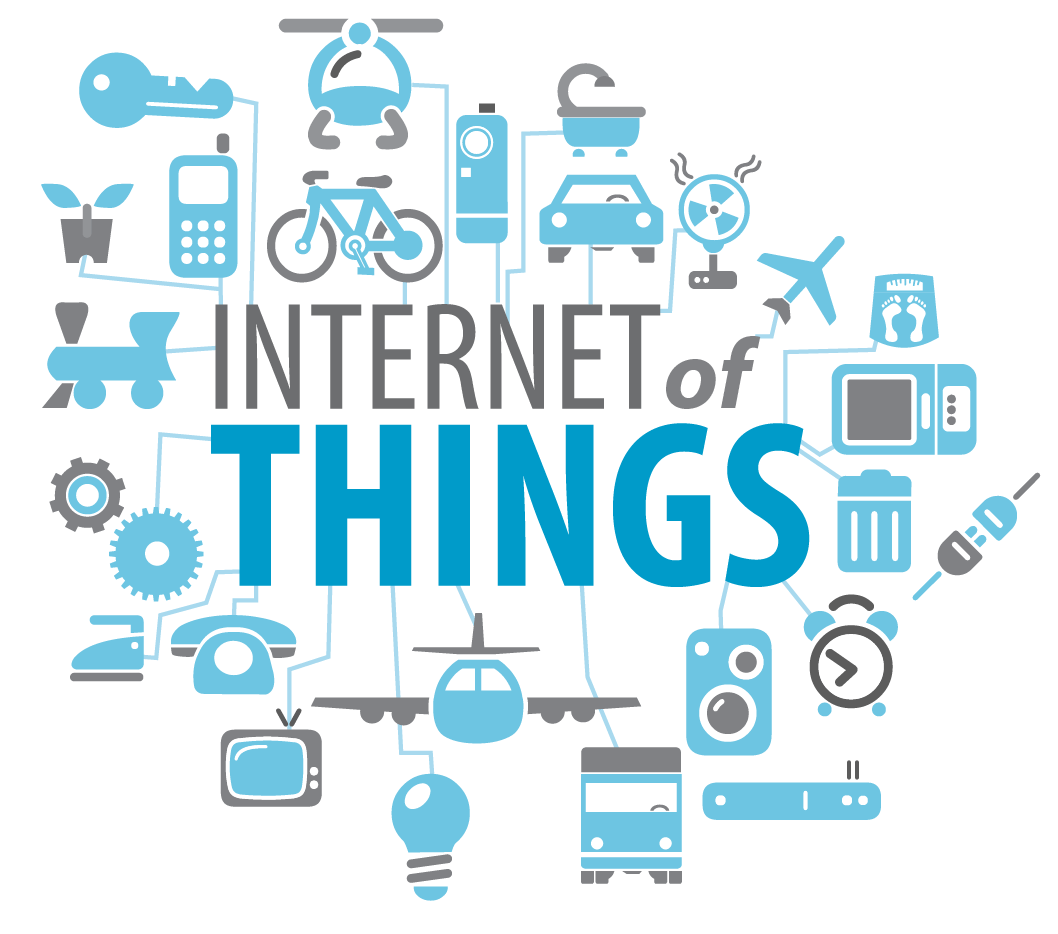
\includegraphics[width=.7\textwidth]{logo}
  \vspace{3cm}
}

\author{Thibaud Besseau, Matthieu Chatelan, Lara Chauffoureaux, Emmanuel Schmid}
\date{\today}

\begin{document}

\maketitle
\thispagestyle{empty}
\clearpage
\tableofcontents
\clearpage
\headsep=20pt

\section{Introduction}
Ce document a pour but la sécurisation du projet élaboré dans le cadre du cours IoT dispensé à la HEIG-VD. Ce dernier est un ....... . Dans ce document, les exigences du projet en général seront décrites ainsi que les biens nécessitant une protection contre tout type de menaces ou tout scénarios d'attaque ainsi que les contre-mesures associées. Toutes les technologies utilisées pour ce projet ont été prises en compte.

\subsection{Equipes}
Lors de ce projet, nous avons créé 5 groupes distincts afin de répartir les différentes compétences et ainsi répartissant la charge de travail pour chacun de ces derniers. Chaucun des groupes avaient un répondant pour les autres groupes (représentés en gras ci-dessous).

\begin{center}
\begin{tabular}{|l|l|}
	\hline
	Groupe & Etudiant \\
	\hline
	Frontend & \textbf{Aurélie Lévy}  \\
	& Tony Clavien\\
	& Mathias Gilson\\
	\hline
	Backend & \textbf{Ludovic Delafontaine}   \\
	& Guillaume Milani\\
	& Sathiya Kirushnpillai\\
	& Mathieu Monteverde\\
	& Nicolas Rod\\
	\hline
	Sécurité & \textbf{Lara Chauffoureaux}  \\
	& Matthieu Chatelan  \\
	& Thibaud Besseau  \\
	& Emmanuel Schmid  \\
	\hline
	Firmware & \textbf{David Truan} \\
	& Théo Gallandat\\
	& Gaëtan Othenin-Girard\\
	& Marie Lemdjo\\
	& Ludovic Richard\\
	\hline
	Infrastructure & \textbf{Julien Brêchet} \\
	& Yosra Harbaoui\\
	& Guillaume Semeels\\
	& Adrien Marco\\
	& Ali Miladi\\
	& Dany Tchente\\
	\hline
\end{tabular}
\end{center}

\newpage
\section{Description du système}

\subsection{Objectifs du système} % description précise du système (nb de capteurs, leur rôles, infra, ...)

Le but de ce système est la collecte de données depuis plusieurs capteurs répartis sur le site de Cheaseaux. Toutes les informations seront consultables sur un frontend accessible par les visiteurs authentifiés sur un compte publique.

Les différents capteurs (voir \autoref{elementssysteme}) se chargent de récolter des informations relatifs à leur environnement et les transmettent à une gateway dont le but est de collecter ces informations des différentes sources. Un bridge assure le lien entre le réseau LORA et le réseau internet standard. Toutes les informations sont finalement transmises à un serveur d'applications sur lequel tourne le backend ainsi que le frontend.

Le schéma ci-dessous illustre cette architecture :

\begin{center}
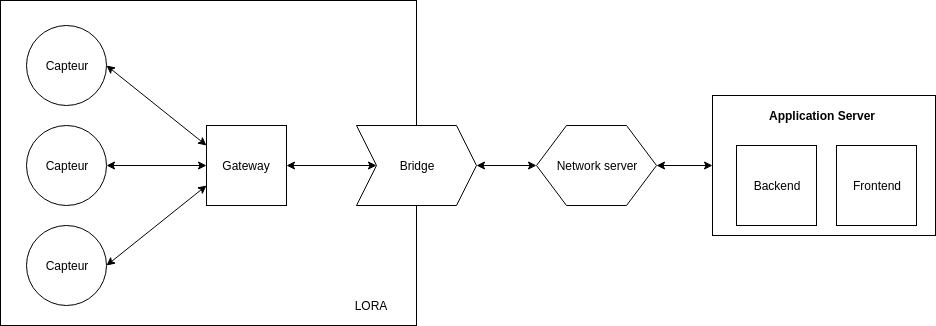
\includegraphics[width=\textwidth]{architecture}
\end{center}

\subsection{Exigences de l'application} % Ce qui est nécessaire pour que l'appli fonctionne + au niveau sécu

L'accès au backend ainsi que l'accès au frontend ne devrait être possible que pour les personnes authorisées et authentifiées à l'aide d'un compte soit utilisateur, soit administrateur.

\subsection{Éléments du systèmes}\label{elementssysteme} % Les différents capteurs, gateways, etc...

Afin de rendre ce système fonctionnel, plusieurs composants hardware ainsi que software doivent être utilisés. En ce qui concerne le hardware, les composants suivants on été utilisés :

\begin{itemize}
	\item Capteurs \\

	\item Gateway \\

	\item Bridge \\
		Dans notre cas lora -> mqtt

	\item Network Server \\

	\item Application Server \\


\end{itemize}

%------------------------ Biens a protéger ---------------------------------
\subsection{Biens nécessitants une protections}
Les biens principaux à sécuriser sont les données transmises entre les différents capteurs et la gateway, ainsi que leur transit vers le serveur d'application et leur utilisation sur ce dernier.


%------------------------ Périmètre sécurisation ---------------------------
\subsection{Périmètre de sécurisation}

%------------------------ Diagramme des flux -------------------------------
\subsection{Diagramme des flux}

%------------------------ Sources de menaces -------------------------------
\section{Sources de menaces}

%------------------------ Début scénarios ----------------------------------
\section{Scénarios d'attaques}
\label{sec:scenarios}

%------------------------ Contremesures ------------------------------------
\section{Contre-mesures}

%------------------------ Conclusion ---------------------------------------
\section{Conclusion}
\label{sec:conclusion}

\end{document}
